\documentclass[tikz,border=15pt]{standalone}
\usepackage[utf8]{inputenc}
\usepackage{tikz}
\usetikzlibrary{shapes,arrows.meta,positioning,calc}

\definecolor{ScoutGreen}{HTML}{005432}
\definecolor{ScoutNavy}{HTML}{002855}
\definecolor{ScoutBlue}{HTML}{006EB6}
\definecolor{ScoutRed}{HTML}{A31920}
\definecolor{ScoutAmber}{HTML}{D97706}
\definecolor{BorderGray}{HTML}{CBD5E1}

\begin{document}
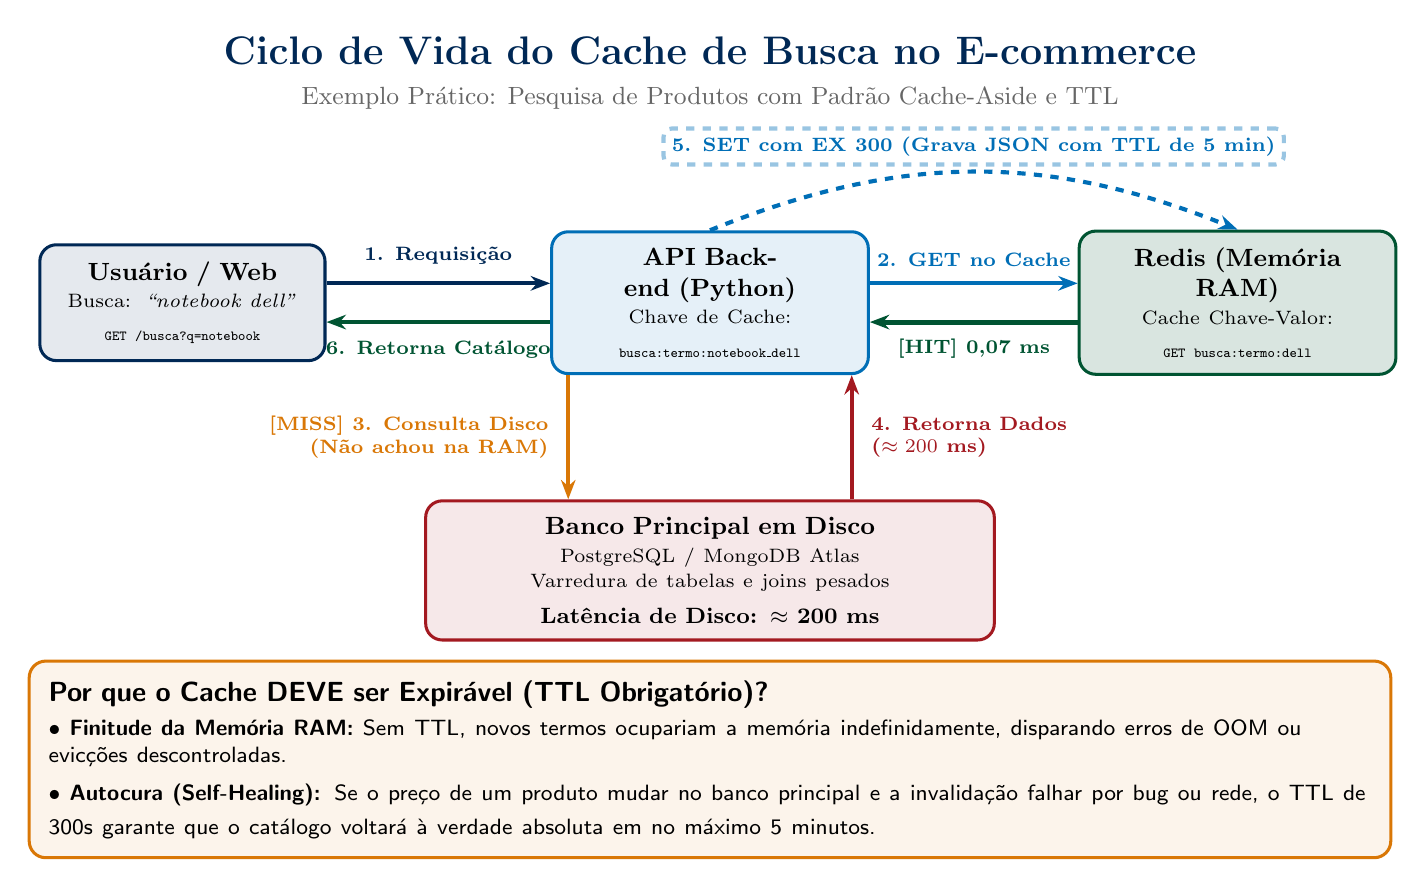
\begin{tikzpicture}[
    font=\sffamily,
    box/.style={draw=BorderGray, rounded corners=6pt, fill=white, line width=1.1pt, align=center, inner sep=6pt},
    arrow/.style={-{Stealth[length=7pt]}, line width=1.4pt}
]

  % =========================================================================
  % CABEÇALHO DO DIAGRAMA
  % =========================================================================
  \node[font=\bfseries\Large, text=ScoutNavy] at (8.5, 8.4) {Ciclo de Vida do Cache de Busca no E-commerce};
  \node[font=\small, text=gray!80!black] at (8.5, 7.8) {Exemplo Prático: Pesquisa de Produtos com Padrão Cache-Aside e TTL};

  % =========================================================================
  % LINHA SUPERIOR: ATORES PRINCIPAIS (ESPAÇAMENTO AMPLO)
  % =========================================================================
  
  % 1. Usuário / Frontend
  \node[box, fill=ScoutNavy!10, draw=ScoutNavy, text width=3.2cm, font=\small] (user) at (1.8, 5.2) {
    \textbf{Usuário / Web}\\[2pt]
    \scriptsize Busca: \textit{``notebook dell''}\\[1pt]
    \tiny \texttt{GET /busca?q=notebook}
  };

  % 2. API Backend
  \node[box, fill=ScoutBlue!10, draw=ScoutBlue, text width=3.6cm, font=\small] (api) at (8.5, 5.2) {
    \textbf{API Backend (Python)}\\[2pt]
    \scriptsize Chave de Cache:\\[1pt]
    \texttt{\tiny busca:termo:notebook\_dell}
  };

  % 3. Redis In-Memory
  \node[box, fill=ScoutGreen!15, draw=ScoutGreen, text width=3.6cm, font=\small] (redis) at (15.2, 5.2) {
    \textbf{Redis (Memória RAM)}\\[2pt]
    \scriptsize Cache Chave-Valor:\\[1pt]
    \texttt{\tiny GET busca:termo:dell}
  };

  % Conexão Usuário <-> API (Espaço de 3.3cm entre caixas)
  \draw[arrow, color=ScoutNavy] ([yshift=7pt]user.east) -- node[midway, above=3pt, font=\scriptsize\bfseries, text=ScoutNavy] {1. Requisição} ([yshift=7pt]api.west);
  \draw[arrow, color=ScoutGreen] ([yshift=-7pt]api.west) -- node[midway, below=3pt, font=\scriptsize\bfseries, text=ScoutGreen] {6. Retorna Catálogo} ([yshift=-7pt]user.east);

  % Conexão API <-> Redis (Espaço de 3.1cm entre caixas)
  \draw[arrow, color=ScoutBlue] ([yshift=7pt]api.east) -- node[above=2pt, font=\scriptsize\bfseries, text=ScoutBlue] {2. GET no Cache} ([yshift=7pt]redis.west);
  \draw[arrow, color=ScoutGreen, line width=1.8pt] ([yshift=-7pt]redis.west) -- node[below=2pt, font=\scriptsize\bfseries, text=ScoutGreen] {\textbf{[HIT]} 0,07 ms} ([yshift=-7pt]api.east);

  % Arco Superior: Gravação no Redis após Miss (Alimentação com TTL)
  \draw[arrow, color=ScoutBlue, dashed, line width=1.5pt] (api.north) to[bend left=22]
    node[midway, above=2pt, font=\scriptsize\bfseries, text=ScoutBlue, fill=white, inner sep=3pt, rounded corners=3pt, draw=ScoutBlue!40] {
      5. SET com EX 300 (Grava JSON com TTL de 5 min)
    } (redis.north);

  % =========================================================================
  % LINHA CENTRAL: BANCO RELACIONAL EM DISCO
  % =========================================================================
  \node[box, fill=ScoutRed!10, draw=ScoutRed, text width=6.8cm, font=\small] (db) at (8.5, 1.8) {
    \textbf{Banco Principal em Disco}\\[2pt]
    \scriptsize PostgreSQL / MongoDB Atlas\\[1pt]
    \scriptsize Varredura de tabelas e joins pesados\\[2pt]
    \footnotesize \textbf{Latência de Disco: $\approx$ 200 ms}
  };

  % Setas verticais para o banco de dados (Miss e Retorno)
  \draw[arrow, color=ScoutAmber, line width=1.6pt] ([xshift=-1.8cm]api.south) --
    node[left=3pt, font=\scriptsize\bfseries, text=ScoutAmber, align=right] {\textbf{[MISS]} 3. Consulta Disco\\(Não achou na RAM)} ([xshift=-1.8cm]db.north);

  \draw[arrow, color=ScoutRed, line width=1.6pt] ([xshift=1.8cm]db.north) --
    node[right=3pt, font=\scriptsize\bfseries, text=ScoutRed, align=left] {4. Retorna Dados\\($\approx 200$ ms)} ([xshift=1.8cm]api.south);

  % =========================================================================
  % FAIXA INFERIOR: POR QUE O CACHE DEVE SER EXPIRÁVEL?
  % =========================================================================
  \node[draw=ScoutAmber, fill=ScoutAmber!8, rounded corners=6pt, text width=16.8cm, align=left, line width=1.1pt, inner sep=7pt] at (8.5, -0.6) {
    \textbf{Por que o Cache DEVE ser Expirável (TTL Obrigatório)?}\\[3pt]
    \footnotesize $\bullet$ \textbf{Finitude da Memória RAM:} Sem TTL, novos termos ocupariam a memória indefinidamente, disparando erros de OOM ou evicções descontroladas.\\[2pt]
    \footnotesize $\bullet$ \textbf{Autocura (Self-Healing):} Se o preço de um produto mudar no banco principal e a invalidação falhar por bug ou rede, o TTL de 300s garante que o catálogo voltará à verdade absoluta em no máximo 5 minutos.
  };

\end{tikzpicture}
\end{document}
